\section{Design}
This section considers the context in which the problem exists and the design of each system and subsystem necessary to visualize and realize a possible solution to solve the problem.

The nature of the system exists primarily in the software domain.
As such, a suitable design architecture is postulated by the C4 model.
This model breaks down the system architecture into different layers of complexity, from a generic high-level system overview down to low-level software abstractions.\cite{vazquez2020c4}

Low-level abstractions are realized with \ac{uml} diagrams. \Ac{uml} diagrams detail the members and methods belonging to classes, and the relationships between those classes in an object-oriented codebase. \cite{petre2013uml}

\subsection{System context and base requirements }
Figure \ref{fig:system_context} depicts the system context in the problem domain.
Project specifications have identified two parties expected to utilize the system - truck drivers and fleet managers.
Identified requirements on the solution dictate that truck drivers will use an android application to log data on the system.
In addition, fleet managers must view the logged data and manipulate their fleets via a web application running in a browser.

\begin{figure}[H]
\centering
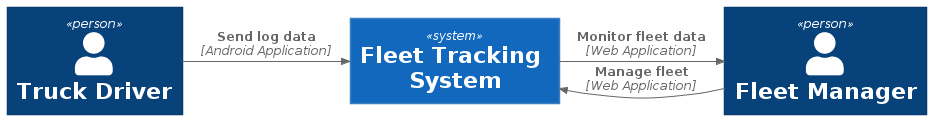
\includegraphics[width=6in]{../diag/system_context.png}
\caption{System Context Diagram}
\label{fig:system_context}
\end{figure}

\begin{figure}
\centering
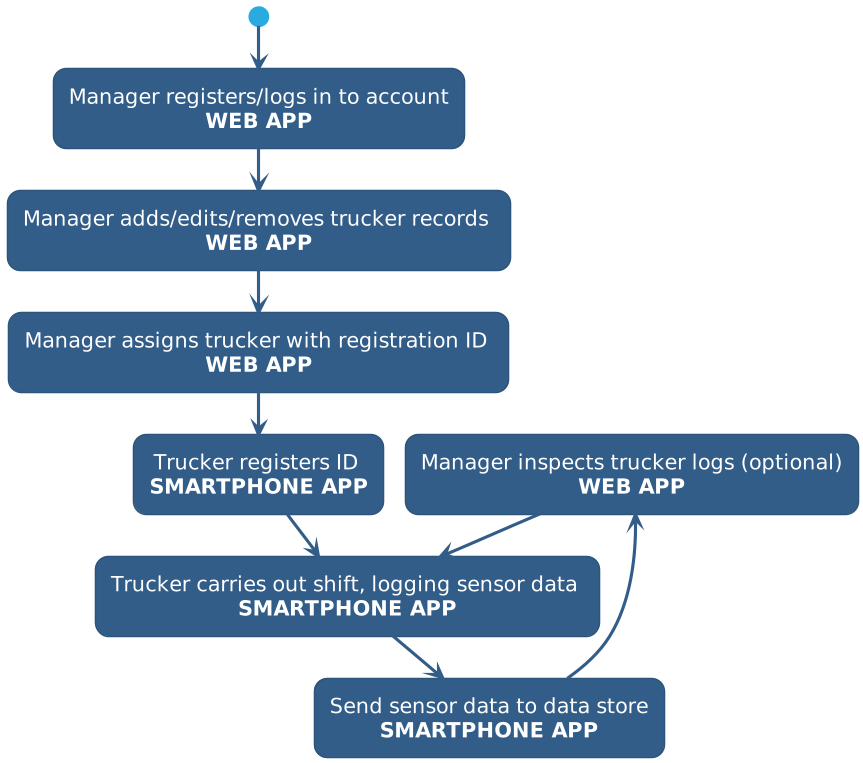
\includegraphics[scale=0.40]{../diag/high_level_activity.png}
\caption{System Lifecycle - High Level}
\label{fig:high_level_activity}
\end{figure}

The high-level life cycle view of the fleet-tracking system design is depicted in figure \ref{fig:high_level_activity}.
This life cycle view gives a broad indication of how the system is expected to work for a user.
Only front-end components of the system are considered to clarify exactly how users will interact with the system.

Managers are required to perform initial configuration, including adding trucker identity records to a data store.
After this, truckers may connect to the system and perform their work while allowing their smartphone applications to track the required sensor data. 
This data is then relayed to the system, in which managers may analyze and inspect data logs.

\subsection{Contained subsystems and choice of technologies}
The second level of the C4 model identifies the choice of technologies to be utilized to realize the fleet tracking system.
The fleet-tracking system is divided into mostly-independent containers, as depicted in figure \ref{fig:container}.
Each container is a standalone process which makes calls to other processes in the system.
The main choice of software tools are identified for each container.

Truckers will make use of an android data-logging application to fetch the various sensor data, and securely transmit this data via an \ac{ssl} connection.
The \ac{io} server, implemented in C++, will listen for multiple asynchronous connections from the android application and relay the data to a MySQL database.
A web application, realized with Microsoft's ASP.NET framework fetches the data and allows the fleet manager to view the whereabouts of each member in his/her fleet.
\begin{figure}[H]
\centering
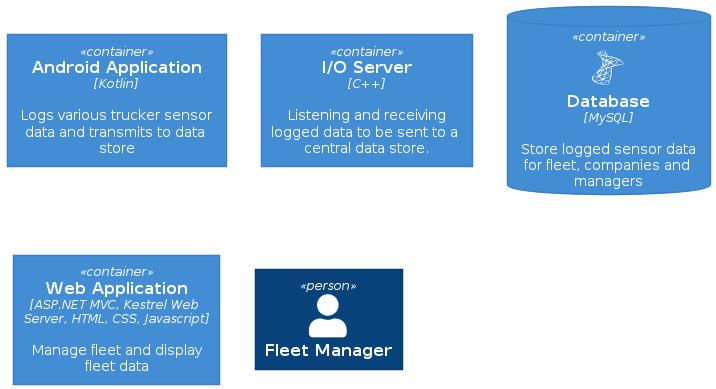
\includegraphics[width=6in]{../diag/container.png}
\caption{Container Diagram - Fleet tracking system}
\label{fig:container}
\end{figure}

\subsubsection{Data Model}
The entire system revolves around the effective abstraction and manipulation of logged fleet data.
MySQL is chosen as the \ac{rdbms} to realize a relational database model, as it is high performance and reliable.
Other \ac{rdbms}s (such as Microsoft SQL Server, PostgreSQL) offer comparable performance, but MySQL is chosen for familiarity.

The relational model is depicted in figure \ref{fig:ERD_Overview}.
The model is designed to allow one company to have many managers and truckers. Each trucker can have many logs.

\subsubsection{Android Application}
Kotlin is the language of choice to write the android application due to its simplicity and mainstream Google support.

Truckers must receive an initial code from their managers' to register their devices.
Sensor readings are taken every two minutes, and stored into a lightweight database.
Finally, a connection is attempted with an \ac{io} server. If available, the database contents is emptied into via the \ac{io} server to the central system database.

\subsubsection{\Ac{io} Server}
C++ is chosen for the \ac{io} server, due to its high performance capabilities.
The \ac{io} server needs to listen and allow multiple asynchronous connections, during which log data is transmitted to the database.

\subsubsection{Web Application}
The \ac{mvc} architecture will be realized with the Microsoft ASP.NET framework.
This architecture allows for separation between business-logic, data models and viewing logic.
This is necessary to ensure that code related to displaying data is not mixed with code used for core logic, thereby separating and modularizing the functionality of different components in the system.

\pagebreak
\subsection{Subsystem components and Design}
Each container in figure \ref{fig:container} is subdivided into several core software components necessary to achieve the desired outcomes.
This is depicted through container diagrams, which makes up the third level of the C4 model.

\subsubsection{Android Application - lifecycle and software abstractions}
\begin{figure}[H]
\centering
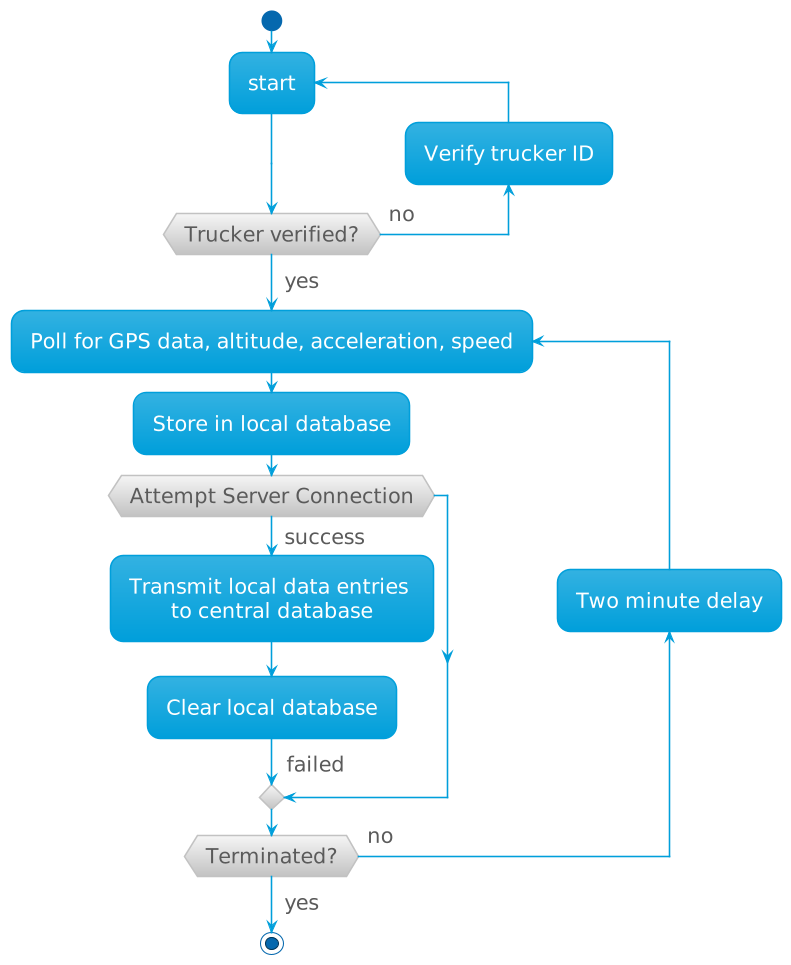
\includegraphics[scale=0.4]{../diag/android_activity.png}
\caption{Life-cycle - Android Application}
\label{fig:android_activity}
\end{figure}

The life cycle of the Android application is depicted in figure \ref{fig:android_activity}.
Initially, a check is performed to confirm that the trucker \ac{id} is in the central database, and is not duplicated.
If this \ac{id} is not valid, the trucker must request a valid \ac{id} from the fleet manager.

After this, the usual logging process is continued.
Data is polled from the available sensors and stored in a local database.
A connection is attempted with the \ac{io} server and the local database entries are transmitted to the server.
Upon successful transmission, the local database is cleared.
However, if a connection fails, the local database is not cleared.
This process loops continuously loops every two minutes.
 
\begin{figure}
\centering
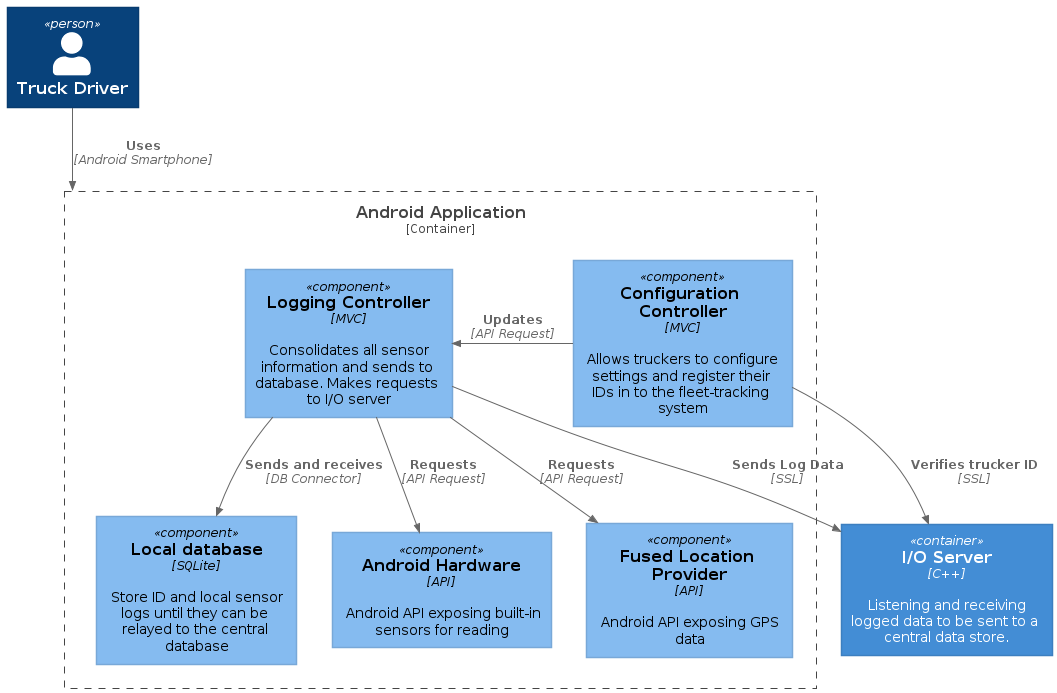
\includegraphics[width=6in]{../diag/android_component.png}
\caption{Component Diagram - Android Application}
\label{fig:android_component}
\end{figure}

The android application is designed with the \ac{mvvm} design pattern (detailed in figure \ref{fig:mvvm_layout}).
Figure \ref{fig:android_component} details software components (classes) that are clearly represented in the source code.
\begin{enumerate}
\item \textbf{Main Activity}\\
The main activity renders the application's main user interface to the user.
This component mainly implements \Ac{ui}-handling logic, with callbacks which are primarily event-driven (when users press buttons for example).
\item \textbf{Main View Model}\\
Activities have short lifetimes and are often recreated when users switch between applications or tilt their screens.
Due to this, a manager class is necessary to ensure data is persisted - this is achieved by the view model.
\item \textbf{Tracking Service}\\
The tracking service is toggleable service which runs in the background as a foreground service.
It polls acceleration and location data via interfaces made available in the Android \ac{api}.
It runs without requiring the main activity to be open on the user's screen.
\item \textbf{Main Repository}\\
Multiple components require performing \ac{io} operations.
To avoid repetition and prevent conflicts, the main repository performs these operations.
It exists as a singleton and is injected into calling objects with \ac{di}.
\item \textbf{Room - Object Relational Mapper}\\
Android's room abstraction layer provides a data class abstraction of data stored in the SQLite database.
This abstraction makes it easier to work with data in language-specific data structures.
Room provides a \ac{dao} to the main repository for database operations.
\item \textbf{SQLite database}\\
SQLite is a lightweight go-to database provider for Android applications.
It is ideal for storing medium to small sized volumes of data.
\item \textbf{Server Connector}\\
The server connector provides \ac{ssl} socket communication with the central \ac{io} server.
Request objects are serialized into text data streams for transmission.
Likewise, server responses are deserialized into response objects and handled appropriately.
\item \textbf{Shared Preferences}\\
Android's \textit{SharedPreferences} library provides an \ac{api} for the purposes of reading/writing key value data in a file on disk.
This is used for storing user configuration, such as identity and upload preferences, which aren't appropriate for a database.
\end{enumerate}

\pagebreak
\subsubsection{\Ac{io} Server}
The typical life cycle view of the \ac{io} server is depicted in figure \ref{fig:IO_activity}.
A secure connection must be made due to the sensitive nature of \ac{gps} data.
\begin{itemize}
\item A session is assigned for the lifetime of the communication, which handles the three-way \ac{ssl} handshake, ensuring the client trusts the server. The incoming payload is decrypted.
\item A request handler parses (and deserializes) the decrypted payload, which queries the database to generate an appropriate serialized response.
\item The response is sent back to the client and the session is terminated.
\end{itemize}

\begin{figure}
\centering
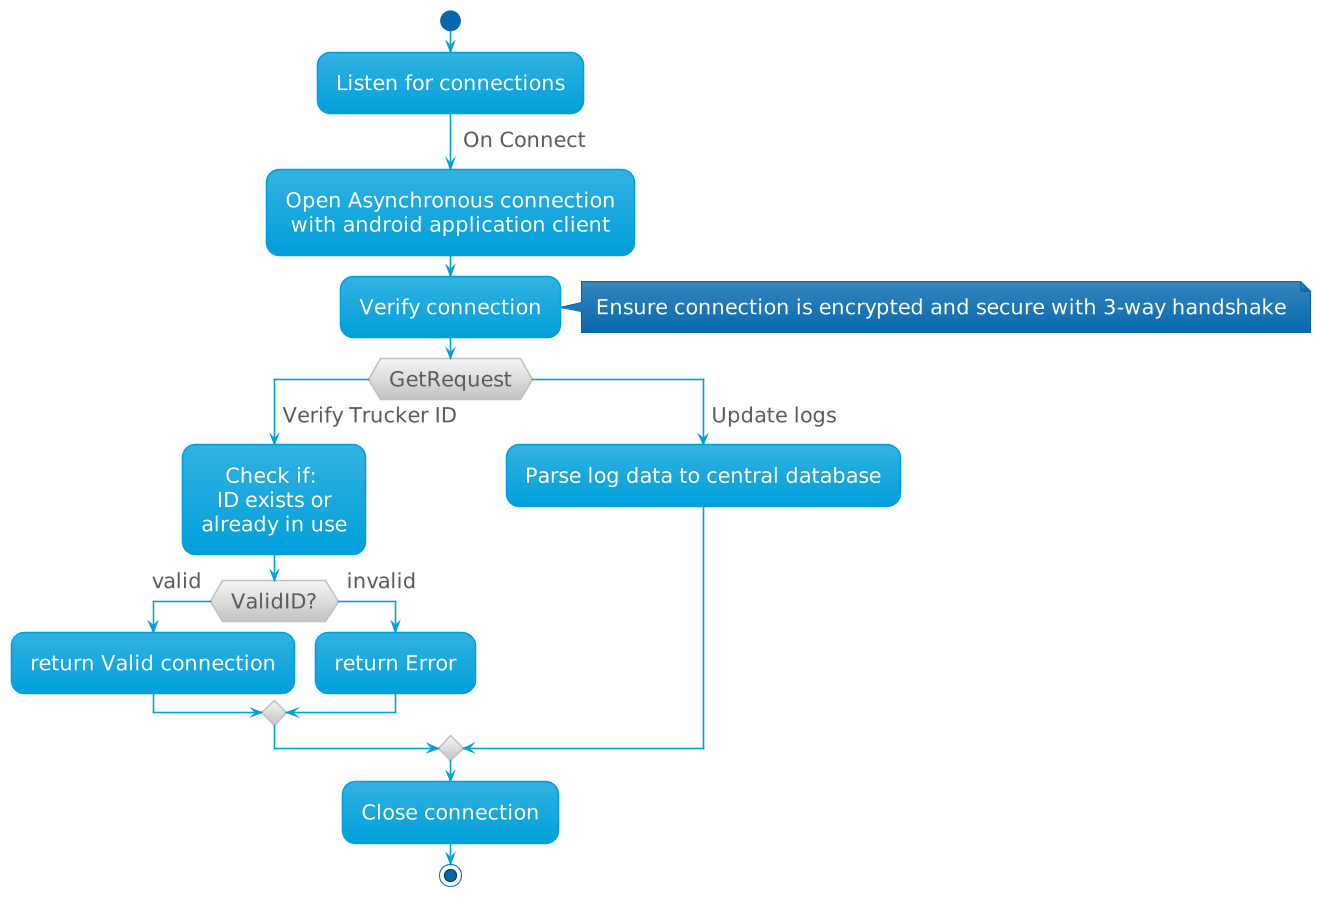
\includegraphics[width=6in]{../diag/IO_activity.png}
\caption{Life cycle - \Ac{io} Server}
\label{fig:IO_activity}
\end{figure}

\begin{figure}[H]
\centering
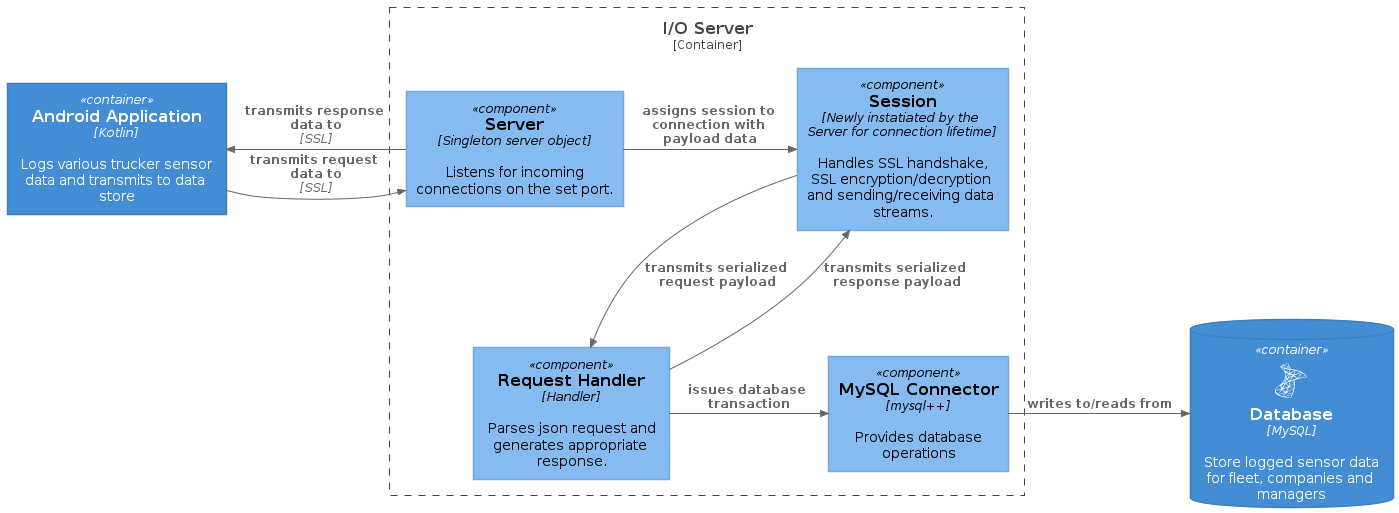
\includegraphics[width=6in]{../diag/IO_component.png}
\caption{Component Diagram - \Ac{io} Server}
\label{fig:IO_component}
\end{figure}

Figure \ref{fig:IO_component} depicts the software abstractions and program structure used to realize the \ac{io} server.
The codebase clearly contains these low-level abstractions.
\begin{enumerate}
\item \textbf{Server}\\
The server object listens for incoming \ac{tcp} connections.
Upon receiving a connection, a new session is instantiated to handle to communication.
\item \textbf{Session}\\
The session performs the necessary encryption, decryption and three-way handshake required for the \ac{ssl} protocol.
The session reads in and writes out the serialized payload on the socket.
\item \textbf{Request Handler}\\
The request handler performs serialization and deserialization.
It processes the request and queries the database appropriately.
\item \textbf{MySQL Connector}\\
An interfacing object to the MySQL database.
\end{enumerate}

\subsubsection{\ac{json} protocol}
\begin{figure}
\centering
    \subfigure[Request payload]
    {
        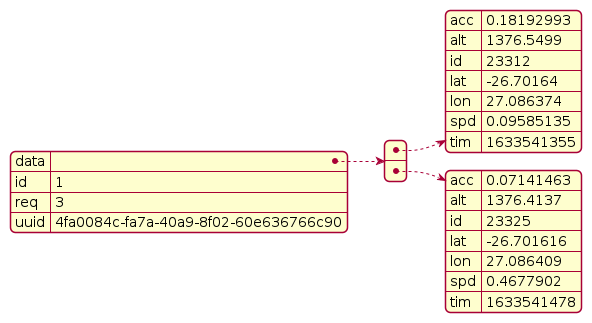
\includegraphics[scale=0.35]{../diag/json_request.png}
        \label{fig:json_request}
    }
    \subfigure[Response payload]
    {
        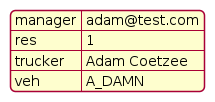
\includegraphics[scale=0.35]{../diag/json_response.png}
        \label{fig:json_response}
    }
\caption{\Ac{json} protocol}
\label{fig:json_protocol}
\end{figure}

\subsubsection{MySQL Database}
The MySQL database is driven by MySQL server.
A relational data structure is utilized, as shown in figure \ref{fig:ERD_Overview}.
Relational modeling allows for logical structuring and integrity of the data.
\begin{figure}
\centering
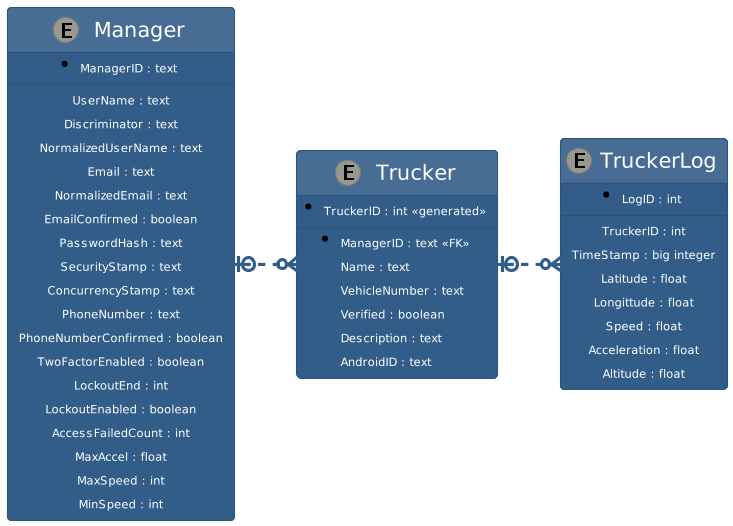
\includegraphics[width=6in]{../diag/erd.png}
\caption{Entity Relationship Diagram}
\label{fig:erd}
\end{figure}

\subsubsection{Web Application}
The web application is modeled with the \ac{mvc} design pattern, which allows separation of \ac{ui} logic from business logic.
Two view models are considered to allow for managers to sign in and manage their fleets.
Controllers handle core logic behind the presentation of data.
The central database is also accessed by the controller.
Figure \ref{fig:webapp_component} depicts the architectural arrangement of the web application.

\begin{figure}
\centering
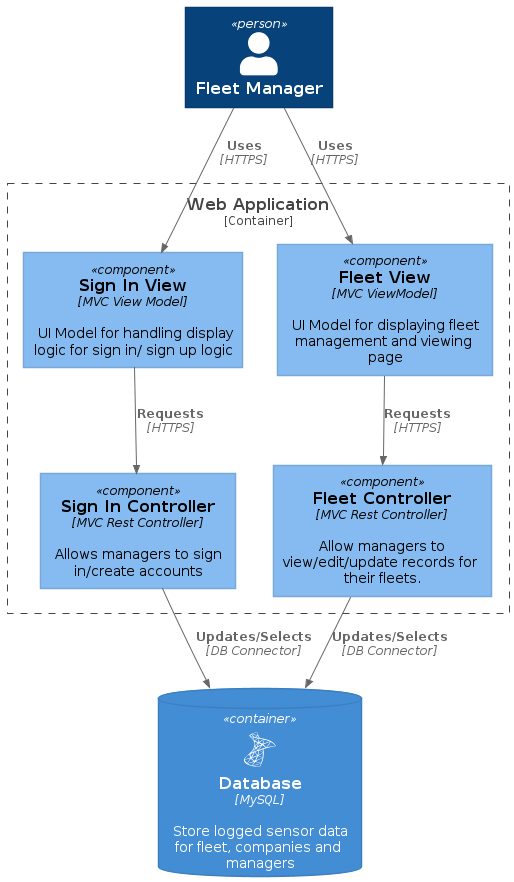
\includegraphics[scale=0.6]{webapp_component.png}
\caption{Component Diagram - Web Application}
\label{fig:webapp_component}
\end{figure}

\pagebreak
